\documentclass[12pt,a4paper]{article}
\usepackage[english, science, large]{../template/ku-frontpage}
\usepackage{tabularx}
\usepackage{ltablex}
\usepackage[cache=false]{minted}
\setminted[erlang]{
frame=lines,
framesep=2mm,
baselinestretch=1.1,
fontsize=\footnotesize,
linenos,
breaklines}
\usemintedstyle{friendly}
\hypersetup{
    colorlinks=false,
    pdfborder={0 0 0},
}
\begin{document}

\title{Quizmaster}
\subtitle{Assignment 5}

\author{Kai Arne S. Myklebust, Silvan Adrian}
\date{Handed in: \today}
	
\maketitle
\tableofcontents

\section{Solution}

\subsection{Files}
All Files are situated in the \textbf{src/} folder:
\begin{itemize}
	\item \textbf{src/quizmaster.erl} The quizmaster Server implementation
	\item \textbf{src/quizmaster\_helpers.erl} The greetings module implementation
	\item \textbf{tests/quizmaster\_conductor.erl} Conductor Implementation for testing
	\item \textbf{tests/quizmaster\_player.erl} Player implementation for testing
	\item \textbf{tests/quizmaster\_tests.erl} Eunit Tests for quizmaster
\end{itemize}

\subsection{Running the programm}
Out of convenience we used a Emakefile which compiles all the erlang files in one go then rather compile each file on it's own.
This can be done by using the erlang shell and run:

\begin{minted}{erlang}
make:all([load]).
\end{minted}

\subsection{Running the tests}
The tests can be run this way:
\begin{minted}{erlang}
eunit:test(quizmaster_tests, [verbose]).
\end{minted}

\section{Implementation}
\subsection{Gen-Statem}
Since the Quizmaster can be seen as a simple State machine we chose gen\_statem.
The Quizmaster has overall 3 important states:
\begin{itemize}
	\item editable
	\item between\_questions
	\item active\_question
\end{itemize} 

\begin{figure}[!htb]
\begin{center}
		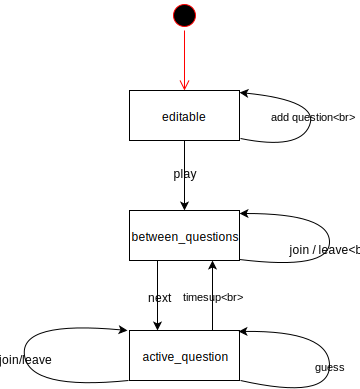
\includegraphics[width=0.65\textwidth]{images/Quizmaster}
\end{center}
	\caption{Simple drawing of the quizmaster state machine}
\end{figure}

\newpage
\subsection{Data Structure}
Data with which we loop is a map with following entries:
\begin{itemize}
	\item \textbf{conductor} The Pid of the Conductor (Gamemaker)
	\item \textbf{questions} all questions which belong to a quiz
	\item \textbf{players} all joined players (we chose to either have active or inactive players (left the game) to get through the tests of OnlineTA)
	\item \textbf{active\_question} The index of the active question (in the questions list)
	\item \textbf{answered} Saving the first guess for each player, to be sure only one guess can be made for each question
	\item \textbf{distribution} the distribution of the current active question which shows which index has be chosen how many times
\end{itemize}

\subsection{All states}
Messages which get accepted in all states.
\subsubsection{get\_questions}
Get all added questions.

\subsection{Editable state}
In the editable state the quiz can be modified, meaning new questions can be added, join is not allowed.

\subsubsection{add\_question}
So the message add\_question adds a new question to the server state, with whom we loop further.
The question does have to in the format:
\begin{figure}
\begin{minted}{erlang}
[Description, [Answers]]
\end{minted}
\caption{Question Format}
\end{figure}

In case the question doesn't fit the format we will get an error back that we tried to add a question in the wrong format, but we don't check if there is a correct answer added (so technically can add a question without any correct answers).
\begin{figure}
\begin{minted}{erlang}
{error, "Question is in wrong format"}
{error, "Wrong Format"}
\end{minted}
\caption{Error Messages}
\end{figure}

\subsubsection{Play}
When all Questions have been added a Quiz can be played, which means it changes it's state to between\_questions and no more questions can be added.
Additionally the Conductor gets set (any process which calls play first).

\subsubsection{Other Messages}
All other messages get ignored in the editable state.

\subsection{Between\_questions state}
In between\_questions new Players can join/leave and the next question can be set to active.

\subsubsection{join}
When joining we check if the nickname already exists, is this is the case then we set the existing player to active again otherwise add it as a new player to the players map in data.
And send a message to the conductor by announcing a new player has joined.

\subsubsection{leave}
When a player leaves the nickname will still exist in the players map, only his status will be set to inactive so that the player still shows in the Report after timesup (this way the distribution still makes sense).

\subsubsection{next}
Select the next active question (according to the index in data), the state also changes to active\_question.
Next can be only called by the conductor, which gets checked against the one saved in data.
Additionally the next question get broadcasted to all joined players, with the Description and the Answers (removing the correct).

\subsubsection{timesup}
Return a error in between\_questions since there is no active question.

\subsection{Active\_question state}
In Active question a player can join or leave, and the players can make guesses. The conductor then can run timesup to finish up the round and change back to between\_questions state.

\subsubsection{join}
Same as in between\_questions.

\subsubsection{leave}
Same as in between\_questions.

\subsubsection{guess}
A guess can be made on a specific index which then either gives a point (if correct answer) or just gets counted into the distribution of the guesses.
If the guess is on a wrong index then the guess is going to be ignored.

\subsubsection{timesup}
Timesup get called by the conductor and only by him, by doing that the state gets changed back to in between\_questions and a reports gets sent out (with distribution, score of all players etc.).
In case it was the last question then all players get a Message with quiz\_over.

\section{Assessment}

\subsection{OnlineTA}
OnlineTA gave ok results back but only the last test wasn't able to fully run through and the end we ended up with guessing what exactly is wished what we implement to get through all test cases, so we gave up in the end.

\subsection{Scope of Test Cases}
We tried to test all possible good and error cases, but to make it a little easier we ignored some of the messages that get sent (see quizmaster\_conductor, quizmaster\_player).
So overall our tests should tests most cases but not all of them.

\subsection{Correctness}
In our opinion, we tested possible edge cases but nonetheless the onlineTA end up in a error in the last test, which we weren't able to find out why.
So the Solution is not fully correct and still seems to miss a few things, but since it would need too much time to fix those we finished it earlier.

\subsection{Code Quality}
There are lots of things which could be made easier in the code, especially lots of duplicated code which could be moved into own helper methods to keep quizmaster.erl more clean.
Especially in this assignment the quizmaster file got quite big and we just tried to make it a little better by moving some functions into the quizmaster\_helpers.erl file.

\appendix
\section{Code Listing}
\inputminted{erlang}{handin/src/quizmaster.erl}
\inputminted{erlang}{handin/src/quizmaster_helpers.erl}

\end{document}